\documentclass[10pt,a4paper]{article}
\usepackage[T1]{fontenc}
\usepackage{lmodern}
\usepackage[margin=22mm]{geometry}
\usepackage{amsmath,amssymb,booktabs,longtable,hyperref,fancyhdr,enumitem,graphicx,pdfpages}
\setlength{\parindent}{0pt}\setlength{\parskip}{.5em}
\setlength{\emergencystretch}{3em}
\pagestyle{fancy}\fancyhf{}
\fancyhead[L]{PCM / GS-PnP SSDU expansion}
\fancyhead[R]{9 November 2026}
\fancyfoot[C]{\thepage}\setlength{\headheight}{14pt}
\begin{document}
{\LARGE\bfseries Expanded GS-PnP SSDU tuning}\\[4pt]
{\large Dedicated preparation and experiment report}\\[4pt]
\textbf{Current status: Completed validation sweep, frozen parameters and retrospective 450-image test.}
\par\medskip\hrule
\section{Executive summary}
The previous ground-truth-free GS-PnP selection was
\(\lambda=0.1\), denoiser \(\sigma=0.075\) and
initial \(\tau_0=100/3\). Each was at the top of
the previous finite search range. The five-image held-out
measurement MSE was 0.0043654339.
We evaluated 27 preregistered candidate configurations, including the
old winning control and 26 previously untested combinations.
Selecting among them must use only archived validation
measurements, never image ground truth or the previously
inspected 450-image test scores.

\section{Tuning algorithm}
Use the same five NPL-noisy validation images:
CIGS 0733, Organic 0008, Perovskite 0283,
Reference 0768 and Silicone 0589.
For each image, retain the first 4,096 coarse rows
of the 13,107 acquired Hadamard measurements in
every reconstruction fold. Divide the remaining
9,011 acquired fine rows into the four previously
frozen disjoint SSDU holdouts.

For candidate \(\theta=(\lambda,\sigma,\tau_0)\),
reconstruct from fit rows \(\Theta_{ik}\)
and score held-out rows \(\Lambda_{ik}\):
\[
L(\theta)=\frac15\sum_{i=1}^{5}\frac14
\sum_{k=1}^{4}
\frac{\|A_{\Lambda_{ik}}\widehat{x}_{\theta,ik}
-y_{\Lambda_{ik}}\|_2^2}{|\Lambda_{ik}|}.
\]
Keep the original normalised PCM operator and summed
half-squared residual fidelity, without a fold-size
rescaling. Use the same pretrained GS-DRUNet and
paper-final \(z\) image.

\subsection*{Frozen parameter grid}
\begin{center}\begin{tabular}{ll}\toprule
Parameter & Candidate values\\\midrule
\(\lambda\) & 0.10, 0.20, 0.40\\
Denoiser \(\sigma\) & 0.075, 0.10, 0.15\\
Initial \(\tau_0\) & 33.3333, 50, 75\\\bottomrule
\end{tabular}\end{center}
Freeze 100 maximum accepted steps, 20 line-search attempts,
\(\gamma=0.1\), \(\eta=0.9\) and stopping
tolerance \(10^{-6}\). Tune \(\lambda\) and \(\tau_0\)
independently. Record accepted iterations,
rejections, final \(\tau\), effective
\(\lambda\tau\), and time per reconstruction.

\section{Step-by-step plan}
\begin{enumerate}[leftmargin=1.5em,itemsep=.2em]
\item Verify the frozen acquisition hashes, original four fold
masks, solver equivalence and data-fidelity scale.
Freeze source hashes and the candidate grid.
\item Reuse the original 20 fold scores of
\texttt{gs\_018} under control ID \texttt{gs\_exp\_001},
keeping original SHA256 provenance.
\item Score 26 new configurations across five images
and four folds: 520 new GS reconstructions.
Each can take up to 100 accepted iterations,
with additional backtracking work.
\item Record all held-out losses and solver diagnostics.
Exclude configurations with any failed fold.
If more than nine candidates fail, withhold selection.
\item Select the minimum balanced SSDU loss,
breaking ties within \(10^{-10}\) by grid order.
Freeze the candidate and every result hash.
\item Check whether the winning parameters are still
at the expanded upper bounds.
Only after freezing, consider a separately labelled
retrospective image-quality comparison.
\item Refresh this report with actual scores and
numerical diagnostics. Do not tune to test PSNR.
\end{enumerate}

\section{Experiment running}
The expanded sweep completed on 9 November 2026. The computing GPU was
tuni's RTX 4090, using an isolated CUDA UUID and
deterministic cuBLAS/cuDNN. The original float64
noisy measurements and mask indices are reused,
while neural solvers receive their required float32
values. The scoring code does not load targets.
Case-level JSON files allow safe resumption.
The old tuned-5 and tuned-50 selection records
and the 450-image test benchmark are preserved.

\section{Results and deliverables}
\input{current_results.tex}
\small
\begin{longtable}{@{}lrrrrl@{}}
\toprule
Candidate&\(\lambda\)&\(\sigma\)&\(\tau_0\)&
SSDU MSE&Status\\\midrule\endfirsthead
\toprule
Candidate&\(\lambda\)&\(\sigma\)&\(\tau_0\)&
SSDU MSE&Status\\\midrule\endhead
\input{candidate_rows.tex}
\end{longtable}
\normalsize
\IfFileExists{figures/candidate_losses.pdf}{\begin{figure}[ht]\centering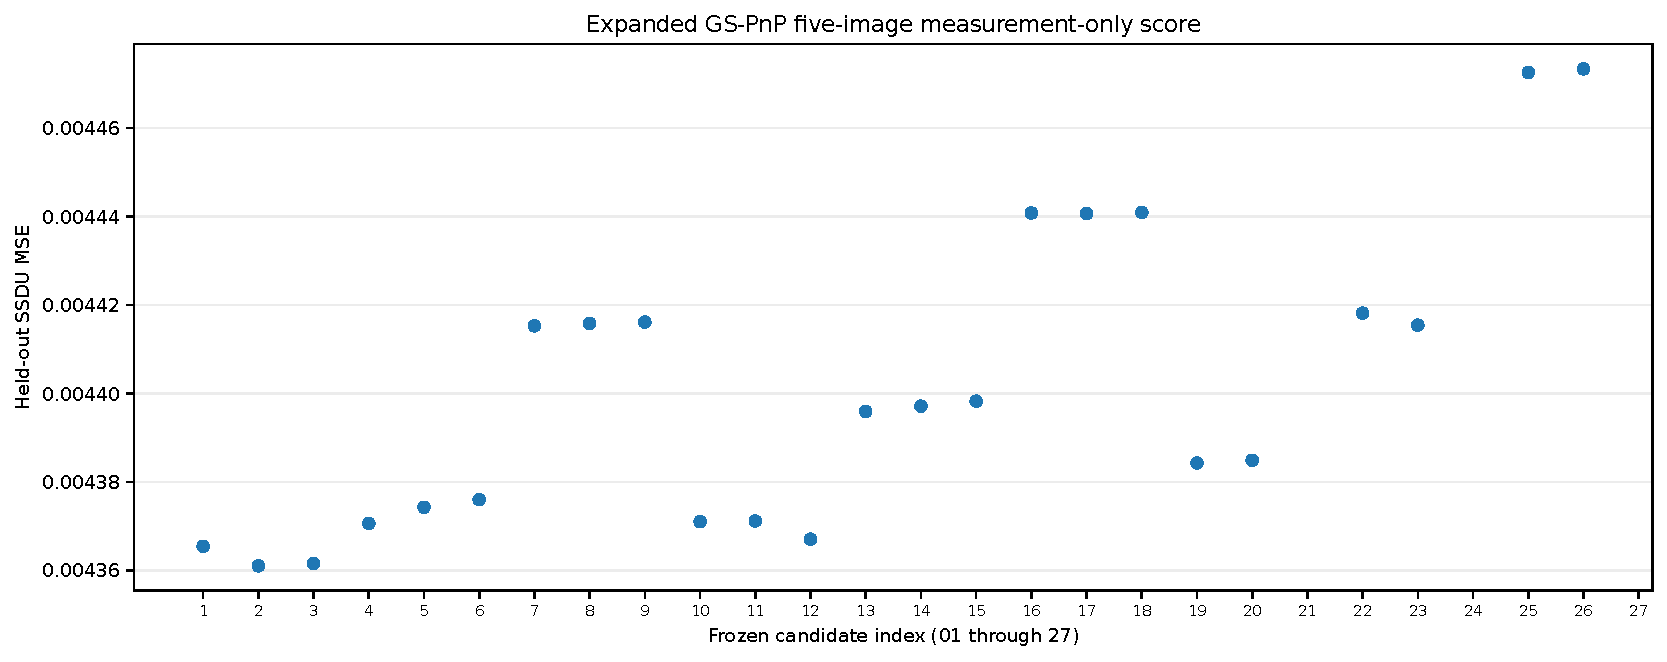
\includegraphics[width=.95\linewidth]{figures/candidate_losses.pdf}\caption{Validation-only SSDU loss across completed candidates.}\end{figure}}{}
\IfFileExists{figures/parameter_slices.pdf}{\begin{figure}[ht]\centering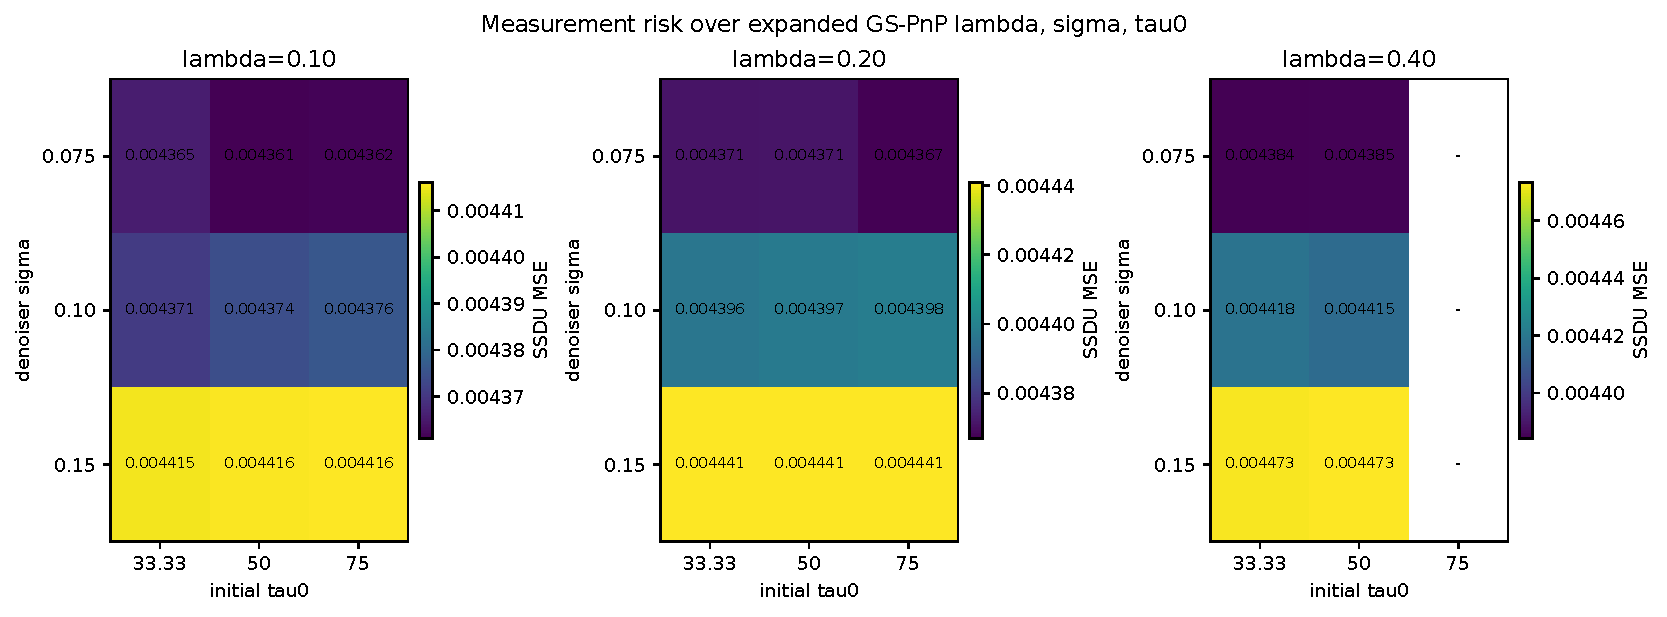
\includegraphics[width=.95\linewidth]{figures/parameter_slices.pdf}\caption{Expanded lambda, sigma and initial step-size slices of the validation-only risk.}\end{figure}}{}
The dedicated folder holds the original grid, preflight,
resumable numerical code, case-level results, frozen selection
and an editable report in both TeX and PDF.


\subsection*{Expanded sweep: measured validation outcome}
The 27 candidates were predeclared before the GPU evaluation.
The original control risk was 0.004365434, while the
minimum validation-only held-out risk was
0.004361004 for \texttt{gs\_exp\_002}.
This is a 0.10 percent reduction in the SSDU loss
relative to the original control. It is a difference in
\emph{measurement prediction error}, not necessarily image
reconstruction quality.

\begin{table}[htbp]
\centering\small
\begin{tabular}{@{}lrrr@{}}
\toprule
Category & Original SSDU MSE & Expanded SSDU MSE & Change\\
\midrule
CIGS & 0.00392860 & 0.00390345 & -0.00002515 \\
Organic & 0.00427257 & 0.00427257 & -0.00000000 \\
Perovskite & 0.00469730 & 0.00469710 & -0.00000020 \\
Reference & 0.00406831 & 0.00406816 & -0.00000015 \\
Silicone & 0.00486039 & 0.00486374 & +0.00000335 \\
\bottomrule
\end{tabular}
\caption{Per-category validation measurement prediction errors: one
image and four held-out folds per category.}
\end{table}

The frozen winning parameters are
\[
\lambda=0.100,\qquad
\sigma=0.075,\qquad
\tau_0=50.0000.
\]
The selection used only the original five validation images
and their fixed holdout masks. No test-image ground truth or
previous test metrics influenced the selection.
There were 3 numerically invalid configurations
out of 27. The winner's upper-bound flags are:
lambda: no, sigma: no, tau0: no.

\begin{table}[htbp]
\centering\small
\begin{tabular}{@{}lll@{}}
\toprule
Invalid candidate & Validation case & Failure reason\\
\midrule
\texttt{gs\_exp\_021} & \texttt{Perovskite\_0283} & No GS iteration accepted \\
\texttt{gs\_exp\_021} & \texttt{Silicone\_0589} & No GS iteration accepted \\
\texttt{gs\_exp\_024} & \texttt{Perovskite\_0283} & No GS iteration accepted \\
\texttt{gs\_exp\_027} & \texttt{Perovskite\_0283} & No GS iteration accepted \\
\bottomrule
\end{tabular}
\caption{Numerically invalid higher-value candidates; they were
excluded rather than silently assigned a favourable SSDU loss.}
\end{table}

\begin{table}[htbp]
\centering\small
\begin{tabular}{@{}lrrrr@{}}
\toprule
\textbf{Candidate}&$\lambda$&$\sigma$&$\tau_0$&\textbf{SSDU risk}\\
\midrule
\texttt{gs\_exp\_002} & 0.100 & 0.075 & 50.000 & 0.00436100 \\
\texttt{gs\_exp\_003} & 0.100 & 0.075 & 75.000 & 0.00436156 \\
\texttt{gs\_exp\_001} & 0.100 & 0.075 & 33.333 & 0.00436543 \\
\texttt{gs\_exp\_012} & 0.200 & 0.075 & 75.000 & 0.00436703 \\
\texttt{gs\_exp\_004} & 0.100 & 0.100 & 33.333 & 0.00437060 \\
\texttt{gs\_exp\_010} & 0.200 & 0.075 & 33.333 & 0.00437101 \\
\texttt{gs\_exp\_011} & 0.200 & 0.075 & 50.000 & 0.00437115 \\
\texttt{gs\_exp\_005} & 0.100 & 0.100 & 50.000 & 0.00437426 \\
\texttt{gs\_exp\_006} & 0.100 & 0.100 & 75.000 & 0.00437598 \\
\texttt{gs\_exp\_019} & 0.400 & 0.075 & 33.333 & 0.00438429 \\
\bottomrule
\end{tabular}
\caption{Top ten valid candidates ranked by frozen five-image SSDU loss.}
\end{table}

\begin{table}[htbp]
\centering\small
\begin{tabular}{@{}lrrrrr@{}}
\toprule
\textbf{Config}&\textbf{Folds}&\textbf{Accepted iters}&
\textbf{Rejections}&$\boldsymbol{\lambda\tau}$&\textbf{s/solver}\\
\midrule
\texttt{gs\_exp\_002} & 20 & 48.0 & 11.8 & 1.466 & 1.054 \\
\texttt{gs\_exp\_001} & 20 & 47.9 & 8.1 & 1.450 & 0.986 \\
\bottomrule
\end{tabular}
\caption{Selected versus original GS control. Means over 20 validation folds.
A faster method may require fewer accepted iterations or less work
per iteration/backtracking.}
\end{table}

\clearpage
\subsection*{Retrospective 450-image PCM evaluation}
After freezing the expanded SSDU winner, we applied it to the
exact same stored fixed 20 percent NPL-noisy acquisitions used
for the previous 450-image comparisons.
For each test image, the sampled Hadamard-mask and noisy
measurement SHA256 hashes were verified against the archived
baseline. We did not select or modify hyperparameters after
examining reconstruction metrics.

The expanded configuration gives mean PSNR 32.563 dB, compared with 32.590 dB for the original SSDU-5 GS-PnP and 35.110 dB for the supervised-validation oracle. The paired expanded-minus-original PSNR difference is -0.027 dB (sample SD 0.531 dB), while the difference against the oracle is -2.547 dB. All test parameters were frozen before scoring these images.

The expanded configuration gave higher PSNR on 349 of 450 matched images, with a median paired change of +0.127 dB. However, 43 images lost over one dB, producing the negative mean paired change despite most cases improving. An eight-case hardware parity audit on the RTX 4090, including large gain and loss cases, reproduced the earlier RTX 4070 original configuration PSNR to within 0.00009 dB. Thus the hardware difference does not explain those selected outliers; full 450-image hardware parity has not been tested.

\begin{table}[htbp]
\centering\scriptsize
\resizebox{\linewidth}{!}{%
\begin{tabular}{@{}lrrrr@{}}
\toprule
\textbf{Method}&\textbf{PSNR, dB}&\textbf{SSIM}&
\textbf{HaarPSI}&\textbf{MSE}\\
\midrule
Zero-filled & 24.97 $\pm$ 1.97 & 0.4823 $\pm$ 0.0527 & 0.5513 $\pm$ 0.0520 & 3.53e-03 $\pm$ 1.62e-03 \\
SPGL1-BP & 25.42 $\pm$ 1.53 & 0.4353 $\pm$ 0.0354 & 0.6452 $\pm$ 0.0772 & 3.06e-03 $\pm$ 1.18e-03 \\
SPGL1-BPDN & 29.37 $\pm$ 3.41 & 0.7161 $\pm$ 0.1036 & 0.6581 $\pm$ 0.0994 & 1.55e-03 $\pm$ 1.18e-03 \\
PnP-ADMM oracle & 35.75 $\pm$ 3.43 & 0.8970 $\pm$ 0.0770 & 0.8814 $\pm$ 0.0619 & 3.54e-04 $\pm$ 2.43e-04 \\
GS-PnP oracle & 35.11 $\pm$ 3.64 & 0.8709 $\pm$ 0.0871 & 0.8628 $\pm$ 0.0735 & 4.18e-04 $\pm$ 2.87e-04 \\
TV & 30.03 $\pm$ 1.94 & 0.7212 $\pm$ 0.0553 & 0.7844 $\pm$ 0.0504 & 1.10e-03 $\pm$ 5.47e-04 \\
UTV-C60 & 32.30 $\pm$ 2.93 & 0.8450 $\pm$ 0.0882 & 0.7699 $\pm$ 0.1101 & 7.28e-04 $\pm$ 4.53e-04 \\
PnP-ADMM tuned-5 & 35.75 $\pm$ 3.43 & 0.8970 $\pm$ 0.0770 & 0.8814 $\pm$ 0.0619 & 3.54e-04 $\pm$ 2.43e-04 \\
GS-PnP tuned-5 & 32.59 $\pm$ 2.70 & 0.7570 $\pm$ 0.0967 & 0.8208 $\pm$ 0.0775 & 6.63e-04 $\pm$ 3.91e-04 \\
GS-PnP expanded-5 & 32.56 $\pm$ 2.65 & 0.7558 $\pm$ 0.0948 & 0.8201 $\pm$ 0.0771 & 6.63e-04 $\pm$ 3.84e-04 \\
\bottomrule
\end{tabular}}
\caption{Mean $\pm$ sample SD over 450 paired images, calculated on
raw (unclipped) reconstructions. Ten method labels are shown,
including the original SSDU-5 and newly expanded-5 GS-PnP.}
\end{table}

\begin{figure}[htbp]
\centering
\includegraphics[width=.95\linewidth]{../test450/analysis/figures/10_methods_450_boxplots.pdf}
\caption{Paired 450-image score distributions for ten methods.
Outliers are not drawn in the boxplot, but all 450 values contribute
to the descriptive statistics.}
\end{figure}

\begin{figure}[htbp]
\centering
\includegraphics[width=.95\linewidth]{../test450/analysis/figures/10_methods_450_mean_sd.pdf}
\caption{Mean and standard deviation for all ten methods across 450 images.}
\end{figure}

\subsection*{Results by device category}
\begin{table}[htbp]
\centering\tiny
\resizebox{\linewidth}{!}{%
\begin{tabular}{@{}lrrrrrrrrr@{}}
\toprule
\textbf{Category}&\textbf{ZF}&\textbf{SPGL1}&\textbf{BPDN}&
\textbf{ADMM}&\textbf{GS oracle}&\textbf{TV}&\textbf{C60}&
\textbf{GS SSDU-5}&\textbf{GS expanded}\\
\midrule
CIGS & 25.71 & 26.49 & 31.10 & 39.30 & 37.89 & 31.16 & 33.04 & 35.31 & 35.25 \\
Organic & 25.49 & 26.37 & 32.05 & 38.90 & 38.94 & 31.50 & 35.72 & 34.96 & 34.83 \\
Perovskite & 27.06 & 26.43 & 31.60 & 35.48 & 35.35 & 31.33 & 32.61 & 31.70 & 31.72 \\
Reference & 24.25 & 24.39 & 26.72 & 32.14 & 31.72 & 28.30 & 29.63 & 29.73 & 29.73 \\
Silicone & 22.34 & 23.44 & 25.38 & 32.95 & 31.65 & 27.87 & 30.49 & 31.25 & 31.27 \\
\bottomrule
\end{tabular}}
\caption{Category mean PSNR in dB; 90 matched test cases per category.
The full ten-method category metrics and their sample standard
deviations are in the companion JSON and figure files.}
\end{table}

\subsection*{Five illustrative PCM reconstructions}
Five example images are shown using exactly the previously fixed case
selection: CIGS 0279, Organic 0331, Perovskite 0786, Reference 0279
and Silicone 0370. Each comparison includes one target and all ten
methods, displaying PSNR, SSIM, HaarPSI and MSE beside the image.
Colour is AFM-hot capped at 0.8, with identical image intensity
range $[0,1]$ for every panel. These examples are illustrative and
were not used to adjust hyperparameters.

\clearpage
\includepdf[pages=-,pagecommand={}]{../test450/analysis/figures/Five_Examples_10_Methods_with_Metrics.pdf}


\section{Conclusion}

The expanded five-image validation SSDU sweep is complete,
and the winning configuration was frozen before the additional
450-image reconstruction evaluation.
The measurement-only SSDU loss fell from 0.004365434 to
0.004361004 (0.10 percent reduction).
The validated candidate is \texttt{gs\_exp\_002}, with
$\lambda=0.100$, $\sigma=0.075$ and
initial $\tau_0=50.0000$.
The selected candidate lies at new upper search bounds
as follows: lambda no, sigma no,
initial step no.

The expanded configuration gives mean PSNR 32.563 dB, compared with 32.590 dB for the original SSDU-5 GS-PnP and 35.110 dB for the supervised-validation oracle. The paired expanded-minus-original PSNR difference is -0.027 dB (sample SD 0.531 dB), while the difference against the oracle is -2.547 dB. All test parameters were frozen before scoring these images.

These observations show the behaviour of this finite,
preregistered SSDU grid. They do not prove a global optimum.
The old test set had already been inspected in the broader
research project, so this is a retrospective controlled test.
Its results must not be used to make further unrecorded
hyperparameter changes. PCM noise correlation and the
undersampled Hadamard nullspace remain important limitations.

\paragraph{Primary papers.}
Yaman et al., \emph{Self-Supervised Learning of
Physics-Guided Reconstruction Neural Networks without
Fully-Sampled Reference Data}, Magnetic Resonance in Medicine
(2020), acquired measurement partitioning:
\url{https://doi.org/10.1002/mrm.28378}.

Hurault, Leclaire and Papadakis,
\emph{Gradient Step Denoiser for Convergent Plug-and-Play},
ICLR (2022), gradient-step update and backtracking:
\url{https://openreview.net/pdf?id=fPhKeld3Okz}.
\end{document}